\section{Directed Graphical Models}
Directed Graphical Models, also known as Bayesian Networks. The joint distribution of a graph with $K$ nodes is given by:
\begin{equation}
    p(x) = \prod_{k=1}^K p(x_k|pa_k)
\end{equation}
where $pa_k$ denotes the set of parents of $x_k$. This is the \textbf{factorization} of a directed graphical model. The learning task is, how to derive join probability distributions to answer questions.

\begin{figure}[tb]
 \centering 
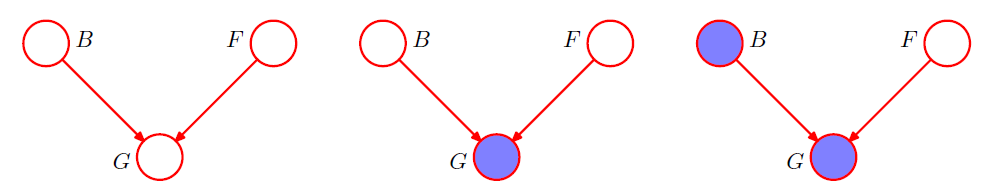
\includegraphics[scale=0.42]{images/DGM.png} 
 \caption{An example of a 3-node graph used to illustrate the phenomenon of ‘explaining away’. The three
nodes represent the state of the battery (B), the state of the fuel tank (F) and the reading on the electric fuel
gauge (G).}
 \label{fig:GDM}
\end{figure}
\textbf{When I turn on the car:} \\
p(B): battery is charged (B=\{0,1\})\\
p(F): there is fuel in the tank (F=\{0,1\})\\
p(G): fuel gauge moves (G=\{0,1\})\\
\\
p(G = 1|B-=1,F=1) = 0.8 \\
p(G = 1|B-=1,F=0) = 0.2 \\
p(G = 1|B-=0,F=1) = 0.2 \\
p(G = 1|B-=0,F=0) = 0.1 \\
p(B=1) = 0.9 \\
p(F=1) = 0.9 \\
From this we can derive: \\
p(G = 0|B-=1,F=1) = 0.2 \\
p(G = 0|B-=1,F=0) = 0.8 \\
p(G = 0|B-=0,F=1) = 0.8 \\
p(G = 0|B-=0,F=0) = 0.9 \\
p(B=0) = 0.1 \\
p(F=0) = 0.1 \\
\textbf{If the gauge does not move, what is the probability that the fuel tank is empty?} \\
\begin{align*}
p(F=0|G=0) & =\frac{p(G=0|F=0)p(F=0)}{p(G=0)} \\
    p(G=0|F=0) & = \sum_{B\in \{0,1\}} p(G=0|B,F=0)p(B) \\
    For B=0: \\
    & = p(G=0|B=0,F=0)p(B=0) \\    
    & = 0.9 * 0.1 \\
    & = 0.09 \\
    For B=1: \\
    &= p(G=0|B=1,F=0)p(B=1) \\   
    & = 0.8 * 0.9 \\
    & = 0.72 \\
p(G=0|F=0) & = 0.09 + 0.72 = \textbf{0.81} \\  
p(F=0) & = \textbf{0.1} \\
p(G=0) & =  \sum_{B\in \{0,1\}}  \sum_{F\in \{0,1\}}  p(G=0|B,F)  p(B)  p(F) \\ 
For B=0, F=0: \\
     & = p(G=0|B=0,F=0)  p(B=0)  p(F=0) \\
    &= 0.9 * 0.1 * 0.1 \\
    & = 0.009 \\
For B=0, F=1: \\
     & = p(G=0|B=0,F=1)  p(B=0)  p(F=1) \\
    &= 0.8 * 0.1 * 0.9 \\
    & = 0.072 \\
For B=1, F=0: \\
     & = p(G=0|B=1,F=0)  p(B=1)  p(F=0) \\
    &= 0.8 * 0.9 * 0.1 \\
    & = 0.072 \\ 
For B=1, F=1: \\
     & = p(G=0|B=1,F=1)  p(B=1)  p(F=1) \\
    &= 0.2 * 0.9 * 0.9 \\
    & = 0.162 \\    
p(G=0) &= 0.009 + 0.072 + 0.072 + 0.162 = \textbf{0.315} \\
p(F=0|G=0) & =\frac{0.81*0.1}{0.315} \\
p(F=0|G=0) & \simeq \textbf{0.257} \\
\end{align*}
Next suppose that we also check the state of the battery and find that it is flat, i.e.,
$B = 0$. The posterior probability that the fuel tank is empty given the observations of both the fuel gauge and the battery state is then given by:
\begin{align*}
    p(F=0|G=0,B=0) = \frac{p(G=0|B=0,F=0)p(B=0)p(F=0)}{\sum_{F\in \{0,1\}p(G=0|B=0,F)p(B=0)p(F)}}
\end{align*}
When expanding the denominator summation, p(B=0) can be factored out and cancelled:
\begin{align*}
    \frac{p(G=0|B=0,F=0)p(B=0)p(F=0)}
    {\big(p(G=0|B=0,F=0)p(F=0) + p(G=0|B=0,F=1)p(F=1)\big)p(B=0)} \\
    \frac{p(G=0|B=0,F=0)p(F=0)}
    {p(G=0|B=0,F=0)p(F=0) + p(G=0|B=0,F=1)p(F=1)}    
\end{align*}
then solved
\begin{align*}
    For F=0: \\
    & = p(G=0|B=0,F=0)p(F=0) \\    
    & = 0.9 * 0.1 \\
    & = 0.09 \\
    For F=1: \\
    & = p(G=0|B=0,F=1)p(F=1) \\    
    & = 0.8 * 0.9 \\
    & = 0.72 \\  
    & = \textbf{0.81} \\      
    p(F=0|G=0,B=0) & = \frac{0.9*0.1}{0.81} \\
    & \simeq \textbf{0.111} 
\end{align*}
In the case of a Naive Bayes Classifier (as a DGM), we again make the assumption of independence:
$$
p(y,\mathrm{x}) = p(y)\prod_{j=1}^Dp(x_j|y)
$$
and would represent the graph likesuch:
\begin{figure}[tb]
 \centering 
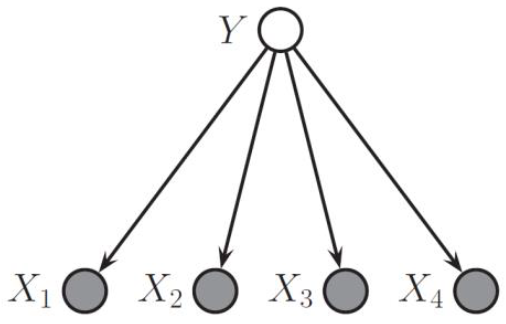
\includegraphics[scale=0.42]{images/bayes-dgm.png} 
 \caption{DGMs - the naive case}
 \label{fig:GDM}
\end{figure}


\begin{align*}
    p(a, b, c) & = p(a)p(c|a)p(b|c) \\
    p(a, b) & = p(a)\sum_c p(c|a)p(b|c) = p(a)p(b|a) \\     
    p(a,b) & = p(b|a)p(a) \\
    p(b|a) & = \frac{p(a,b)}{p(a)} \\
    p(a, b) & = p(a)\sum_c p(c|a)p(b|c) \\
    \sum_c p(c|a)p(b|c) & = \frac{p(a,b)}{p(a)}  = p(b|a) \\
    p(a, b) & = p(a)\sum_c p(c|a)p(b|c) = p(a)p(b|a) \\ 
\end{align*}

Another bayesian abomination: \\

\begin{align*}
p(a,b|c) & = \frac{p(a,b,c)}{p(c)} \\
 & = \frac{p(a)p(c|a)p(b|c)}{p(c)}\\
 & = \frac{p(a)\frac{p(a|c)p(c)}{p(a)}p(b|c)}{p(c)}\\
 & = \frac{p(a|c)p(c)p(b|c)}{p(c)}\\ 
 & = p(a|c)p(b|c)\\  
\end{align*}


Next we look at "A Simple Example" of Bayesian Networks given in class: \\
\textbf{1. The facts}\\
A is "Mike is not answering his phone" \\
B is "Mike is at home"\\
C is "It is raining"\\
\textbf{The fact dependencies} \\
\begin{figure}[H]
 \centering 
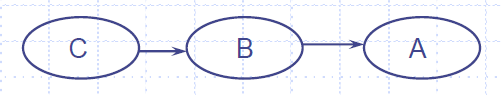
\includegraphics[scale=0.42]{images/mike-phone.png} 
 \caption{Directed graph - simple example}
 \label{fig:Mike}
\end{figure}
Note: C affects A indirectly in this case, so they can be treated as independent! \\
Let:
\begin{align*}
 P(A|B)& = 0.1 \\
 P(A|\midtilde B) & = 1 \\
P(B|C) & = 0.8 \\ 
P(B|\midtilde C) & = 0.5 \\
P(C) & = 0.6    \\
\end{align*}
from which we may further derive:
\begin{align*}
 P(\midtilde A|B)& = 0.9 \\
P(\midtilde B|C) & = 0.2 \\ 
P(\midtilde  B|\midtilde C) & = 0.5 \\
P(\midtilde  C) & = 0.4    \\
\end{align*}
\textbf{The probability that it is raining and Mike is at home but not answering the phone:} \\
\begin{align*}
p(A,B,C) & = p(A|B)p(B|C)p(C) \\
p(A,B,C) & = 0.1 * 0.8 * 0.6 \\
p(A,B,C) & = 0.048 \\
\end{align*}
Other possible calculations…\\
1. Calculate any of the dependent probabilities\\
\textbf{e.g. the probability that Mike is not answering the phone: P(A) = ?} \\
\begin{align*}
    p(A) & = p(A|B)p(B) + p(A|\midtilde B) p(\midtilde B) \\
\end{align*}
We have $p(A|B), p(A|\midtilde B)$, we don't have $p(B), p(\midtilde B)$.
\begin{align*}
    p(B) & = p(B|C)p(C) + p(B|\midtilde C)p(\midtilde C) \\
    p(B) & = 0.8*0.6 + 0.5*0.4 \\
    p(B) & = 0.68 \\
    p(\midtilde B) & = 0.32 \\
\end{align*}
Now we can solve:
\begin{align*}
    p(A) & = p(A|B)p(B) + p(A|\midtilde B) p(\midtilde B) \\
    p(A) & = 0.1*0.68+1*0.32 \\
    p(A) & = 0.388 \\
\end{align*}
2. Compute the probability of some event given the evidence\\
\textbf{e.g. the probability that it is raining given that Mike isn’t answering the phone: P(C|A) = ?} \\
\begin{align*}
    p(C|A) & = \frac{p(A,C)}{p(A)} \\
    % p(C|A) & = \frac{p(A|C)P(C)}{p(A)} \\
    % p(C|A) & = \frac{p(A|C)P(C)}{p(A)} \\
\end{align*}
%We have $p(C),p(A)$, we don't have $p(A|C)$. We derive it from the joint probability:
We have $p(A)$, we don't have $p(A,C)$:
\begin{align*}
    p(A,C) & = \sum_B p(A|B)p(B|C)p(C) \\
    p(A,C) & = p(A|B)p(B|C)p(C) + p(A|\midtilde B)p(\midtilde B|C)p(C) \\
    p(A,C) & = 0.1*0.8*0.6+1*0.2*0.6 \\
    p(A,C) & = 0.168 \\
    p(C|A) & = \frac{0.168}{0.388} \\
    p(C|A) & = 0.433 \\
\end{align*}
3. Compute the most likely set of events, given the evidence \\
\textbf{e.g. What is the most likely explanation for Mike not answering the phone?} Mike not answering the phone is the prior, so we want a likelihood (e.g. Mike is not at home) \textit{given Mike is not answering his phone...}, that is, given a prior.\\
\begin{align*}
p(B|A) & = \frac{p(A|B)p(B)}{p(A)} \\
p(B|A) & = \frac{0.1*0.68}{0.388} = 0.1753\\
p(\midtilde B|A) & = 1 - p(B|A) = \textbf{0.8247} \\
p(C|A) & = 0.433 \\
p(\midtilde C|A) & = 1 - p(C|A) = 0.567 \\
p(B,C|A) & = \frac{p(A,B,C)}{p(A)} = \frac{0.048}{0.388} = 0.1237 \\
p(\midtilde B, C|A) & = \frac{p(A,\midtilde B,C)}{p(A)}  = \frac{p(A|\midtilde B)p(\midtilde B|C) p(C)}{p(A)} = \frac{1*0.2*0.6}{0.388} = 0.3093\\
p(B, \midtilde C|A) & = \frac{p(A,B,\midtilde C)}{p(A)}  = \frac{p(A|B)p(B|\midtilde C) p(\midtilde C)}{p(A)} = \frac{0.1*0.5*0.4}{0.388} = 0.0515 \\
p(\midtilde B, \midtilde C | A) & = \frac{p(A,\midtilde B,\midtilde C)}{p(A)}  = \frac{p(A|\midtilde B)p(\midtilde B|\midtilde C) p(\midtilde C)}{p(A)} = \frac{1*0.5*0.4}{0.388} = 0.5155 \\
\end{align*}
The most likely explanation Mike is not answering the phone, is $p(\midtilde B|A)$, that is to say \textit{Mike is not at home, given he is not answering his phone}.

